\chapter{Background Prediction}
\begin{section}{Overview}

This analysis seeks to find evidence of new physics by searching for deviations from the SM in the \Nb distribution.
In order to do this, it is essential to be able to robustly and accurately predict both the normalization and shape of the \Nb distribution.
To obtain these predictions, a global maximum-likelihood fit is performed.
This fit is carried out both for a background-only hypothesis and for signal-plus-background hypotheses, in which a signal contribution is extracted in addition to the contributions of SM background processes.
The model is constructed using the poisson probabilities of the bin contents of the \Nb distribution for all \Njets, \MJ regions, while systematic uncertainties are applied as nuisance parameters.

As the kinematic tails of the \Njets and \MJ variables are difficult to model reliably, the \ttbar and QCD normalizations are individually allowed to (almost) freely vary in each (\Njets, \MJ) bin.
The \ttbar normalizations are constrained in each bin by the low-\Nb bins, while the QCD normalizations are constrained by control regions with no identified leptons ($\Nleps = 0$).
The overall \Wjets normalization is determined from data and is allowed to vary across \Njets bins by amounts measured using a kinematically similar \Zjets sample, while the normalization of Other is largely taken from simulation, as its contribution is small in the regions considered.
Further details on the measurement of the normalizations are given in the following sections.

Once the SM backround processes are normalized accordingly, further corrections to the \Nb shape are relatively small.
The nominal \Nb shape prediction for each process is taken from simulation with data-to-simulation correction factors (SFs) applied for the tagging efficiency of heavy- and light-flavor jets~\cite{Chatrchyan:2012jua,BTV-16-002}.
This shape is allowed to vary in order to assess the impact of mismodeling of relevant parameters, such as the rate of gluon splitting to \bbbar and the b-tagging SFs.
The appropriate ranges for these parameters are determined based on measurements in dedicated control samples and then constrained by a simultaneous fit across all bins of \Njets and \MJ in a correlated manner.
A detailed discussion of these variations and their measurements is given in~\ref{Systematis Uncertainties}.

\end{section}

\begin{section}{\ttbar and QCD Normalizations}

The \ttbar and QCD normalizations are allowed to float in each (\Njets, \MJ) bin but with a loose constraint across \MJ bins discussed in the following subsection.
The largest constraint on the \ttbar normalization in each bin is the background-dominated $\Nb \leq 2$ bins, while the QCD normalization in each bin is mostly constrained by corresponding bins in a similar 0-lepton kinematic region selected by requiring $\Nleps = 0$, $\HT > 1500~\GeV$, $\MJ > 500~\GeV$, $\Njets \geq 6$, and $\Nb \geq 1$.
The higher \HT requirement compared to the analysis's baseline selection is imposed in order to account for the extra energy in an event carried by the lepton in the $\Nleps = 1$ selection, while the higher \Njets selection is imposed in order to account for differences in the \Njets distribution between the $\Nleps = 1$ and $\Nleps = 0$ samples.
This control sample follows the same kinematic binning as the $\Nleps = 1$ regions, except that the \Nb distribution in each bin is integrated in \Nb for $\Nb \geq 1$ and each bin's \Njets requirement is increased by 2.
A diagram representing the binning of the $\Nleps = 0$ control sample is shown in Figure~\ref{fig:nlep0_regions}
The QCD contribution in a particular $\Nleps = 1$ bin is then constrained by the corresponding $\Nleps = 0$ bin.
To avoid biasing the normalization measurement, the small contribution of \ttbar background to the $\Nleps = 0$ control regions is included using the normalization from the corresponding $\Nleps = 1$ bins, while contributions from other processes are taken from simulation.

\begin{figure}[tbp!]
\centering
\begin{tabular}{ |c|c|c|c| }
\hline
%\multirow{2}{*}{\MJ [\GeV]} & \multicolumn{3}{c|}{\Njets} \\ \cline{2-4}
%                                     & 4--5                & 6--7  & $\geq$8   \\ \hline
%500--800                             & CR                  & CR    & SR        \\ \hline
%800--1000                            & \multirow{2}{*}{CR} & SR    & SR        \\ \cline{1-1} \cline{3-4}
%$>$1000                              &                     & SR    & SR        \\ \hline
\end{tabular}
\caption{Diagram depicting the (\Njets, \MJ) binning of the $\Nleps = 0$ QCD control region.}
\label{fig:nlep0_regions}
\end{figure}

\begin{subsection}{\MJ Connection}

Due to the large freedom of unconstrained normalization parameters, the fit can be sensitive to rare statistical fluctuations and return unphysical normalization values particurlarly in bins dominated by \ttbar events.
For example, in psuedodata experiments, where data are generated according to the statistical and systematic uncertainties of the pre-fit values, the fit reduced the \ttbar contribution in the $\Njets \geq 8$, $\MJ > 1000~\GeV$ bin (where statistical uncertainties are largest) to $\sim0$ in about $\sim1\%$ of the experiments.
This can be seen in Figure~\ref{fig:mj_connection_exps} (left) which shows a low tail in the distribution of post-fit \ttbar yields in the $\Njets \geq 8$, $\MJ > 1000~\GeV$ bin for 1,000 psuedodata experiments.
When yields in a bin have a large fluctuation downwards, the fit must lower the normalization of a process to compensate.
The QCD, \Wjets, and Other contributions, however, are largely constrained by other data control samples or taken from simulation, and so the fit uses the freedom to adjust the \ttbar normalization in order to compensate for the fluctuation, leading to the unphysically small values.

In order to avoid this instability, the normalizations of \ttbar and QCD are (independently) connected by log-normal constraints between adjacent \MJ bins.
By correlating the normalizations across \MJ bins, the fit's sensitivity to large fluctuations in a single bin is greatly reduced.
The size of these connections is motivated by measurements of the data-to-simulation ratio with $\Nb = 1$ events (in order to avoid potential signal contamination) and is particuarly chosen to be significantly larger than the uncertainty on the data-to-simulation ratios in order to avoid over-constraining the normalization parameters, while still providing some constraint against unphysical fits.
Based on these measurements, shown in Figure~\ref{fig:mj_connection}, and criteria, a connection size between adjacent bins of [50\%-200\%] is chosen.

Figure~\ref{mj_connection_exps} (right) shows the results of the same 1,000 psuedodata experiments but now with this constraint across \MJ bins applied.
The resulting distribution of post-fit \ttbar yields now shows no evidence of unphysical normalizations and appears to be better behaved.

\begin{figure}[tbp!]
\centering
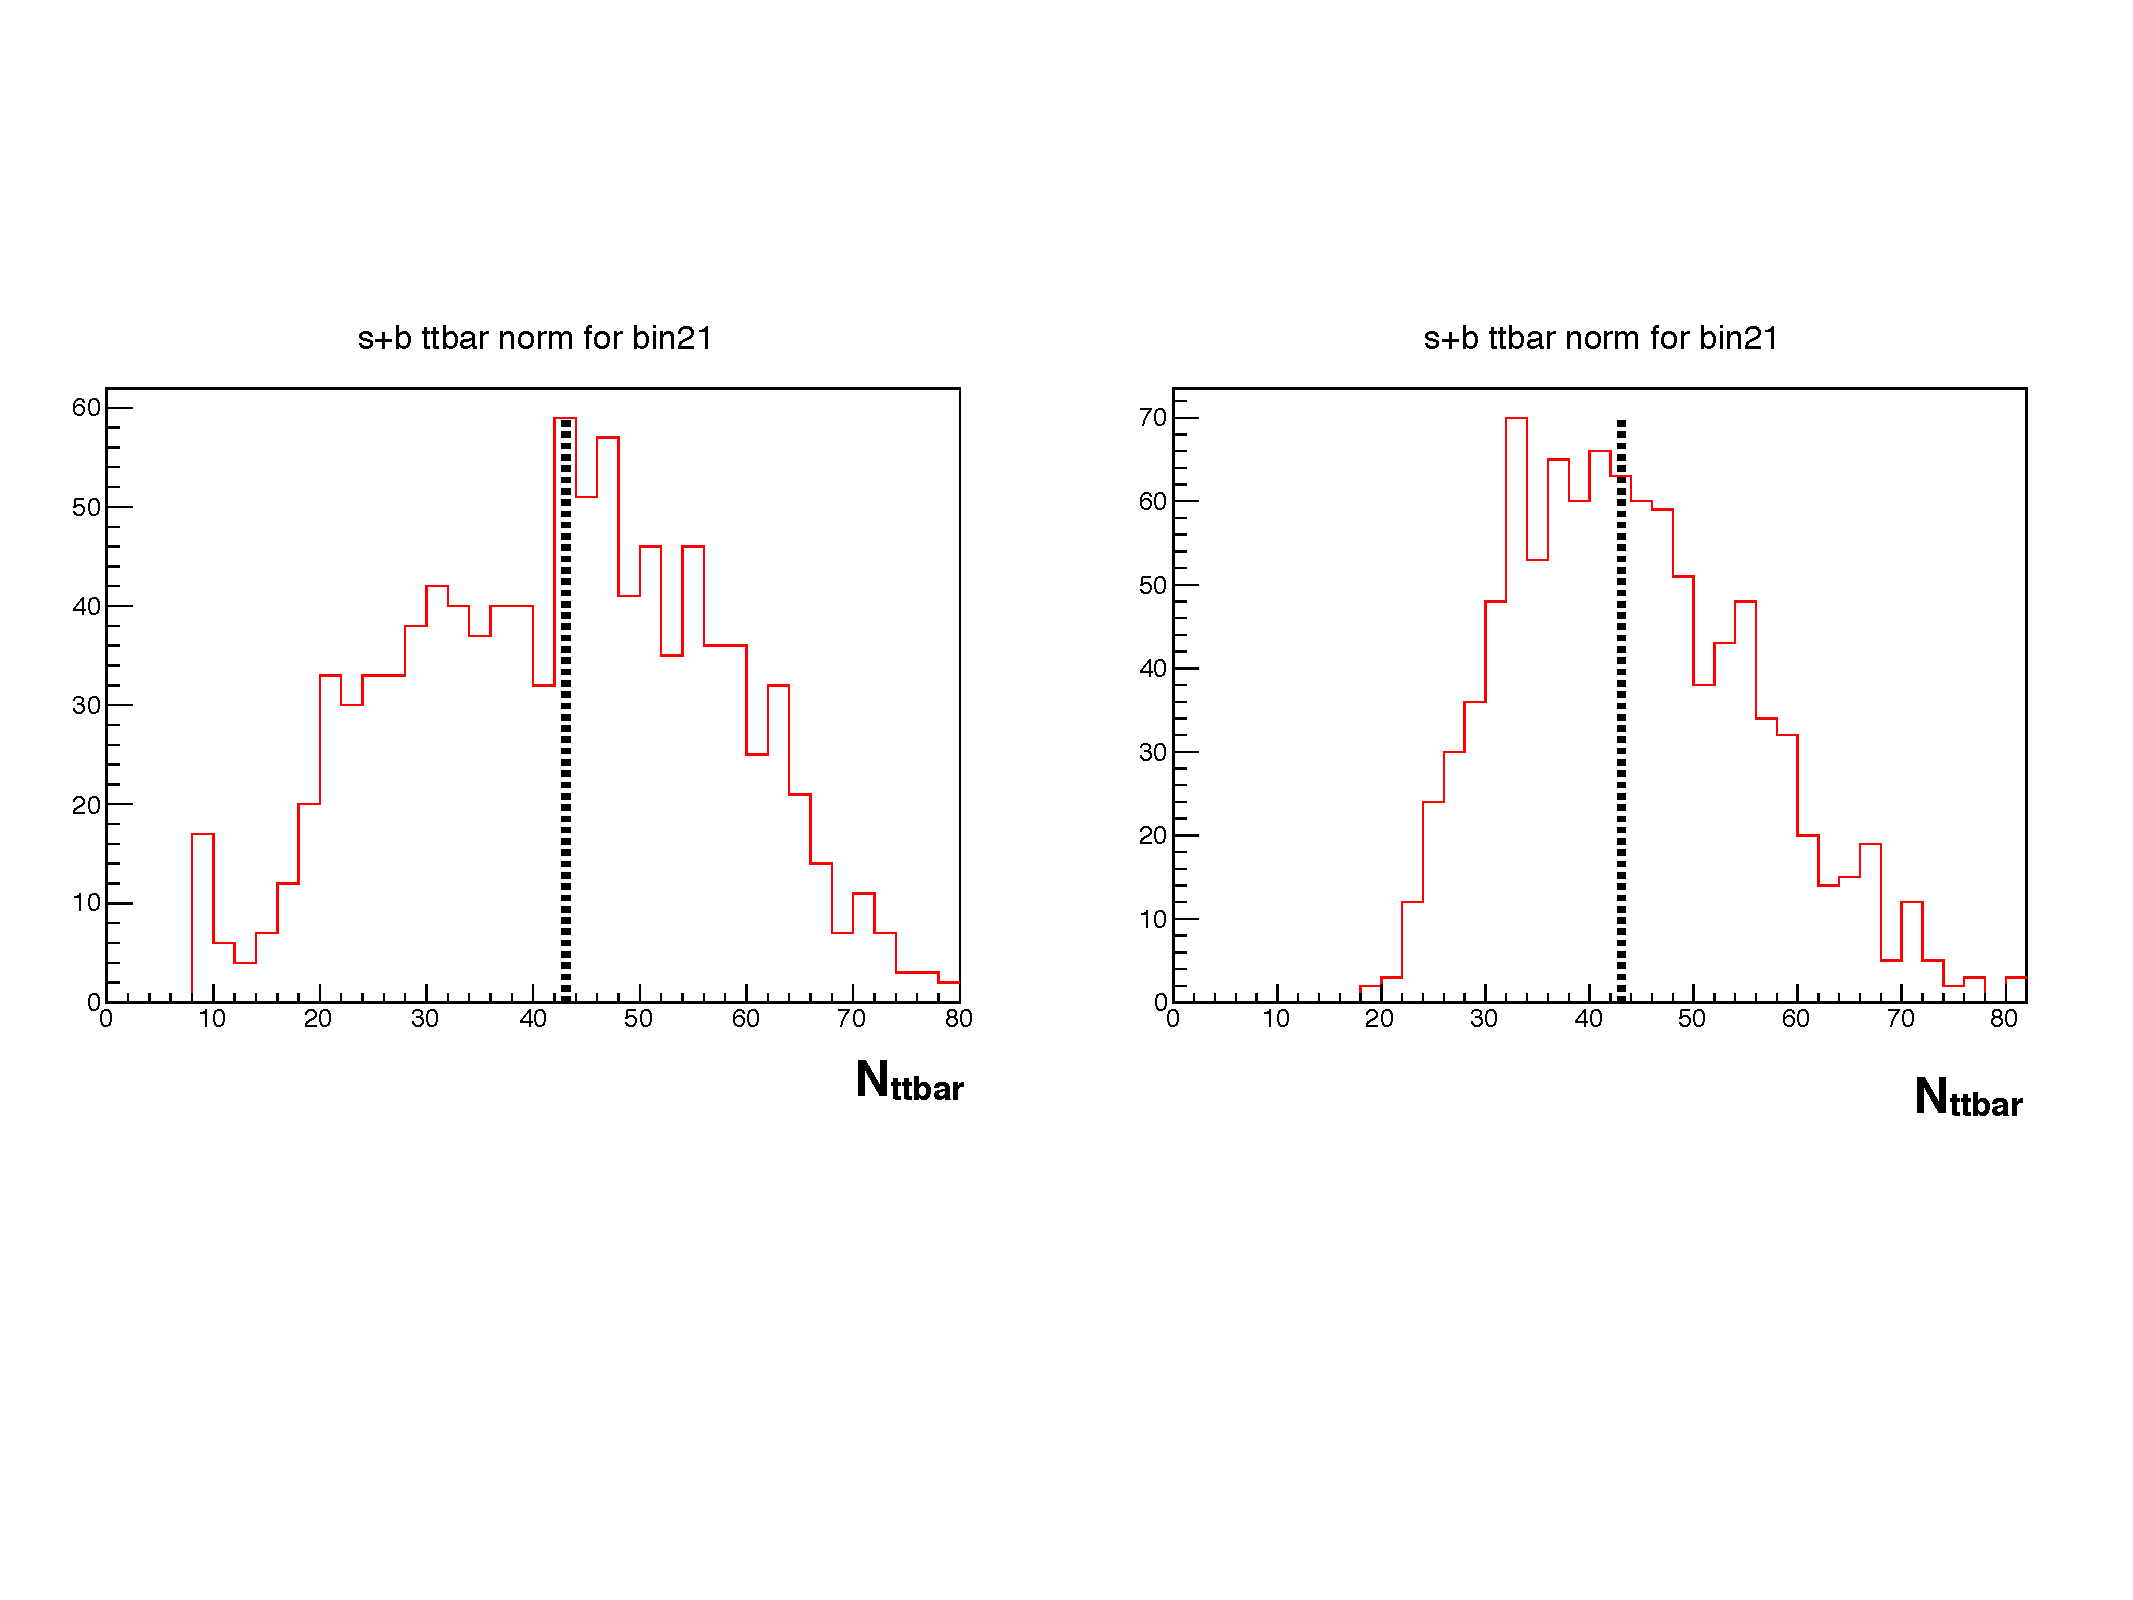
\includegraphics[angle=0,width=0.90\columnwidth]{fig/mj_connection_exps.pdf}
\caption{Distribution of post-fit yields of \ttbar in the $\Njets \geq 8$, $\MJ > 1000~\GeV$ bin for 1,000 psuedodata experiments without (left) and with (right) constraints between adjacent \MJ bins.
The dotted black line indicates the the pre-fit yield.}
\label{fig:mj_connection_exps}
\end{figure}

\begin{figure}[tbp!]
\centering
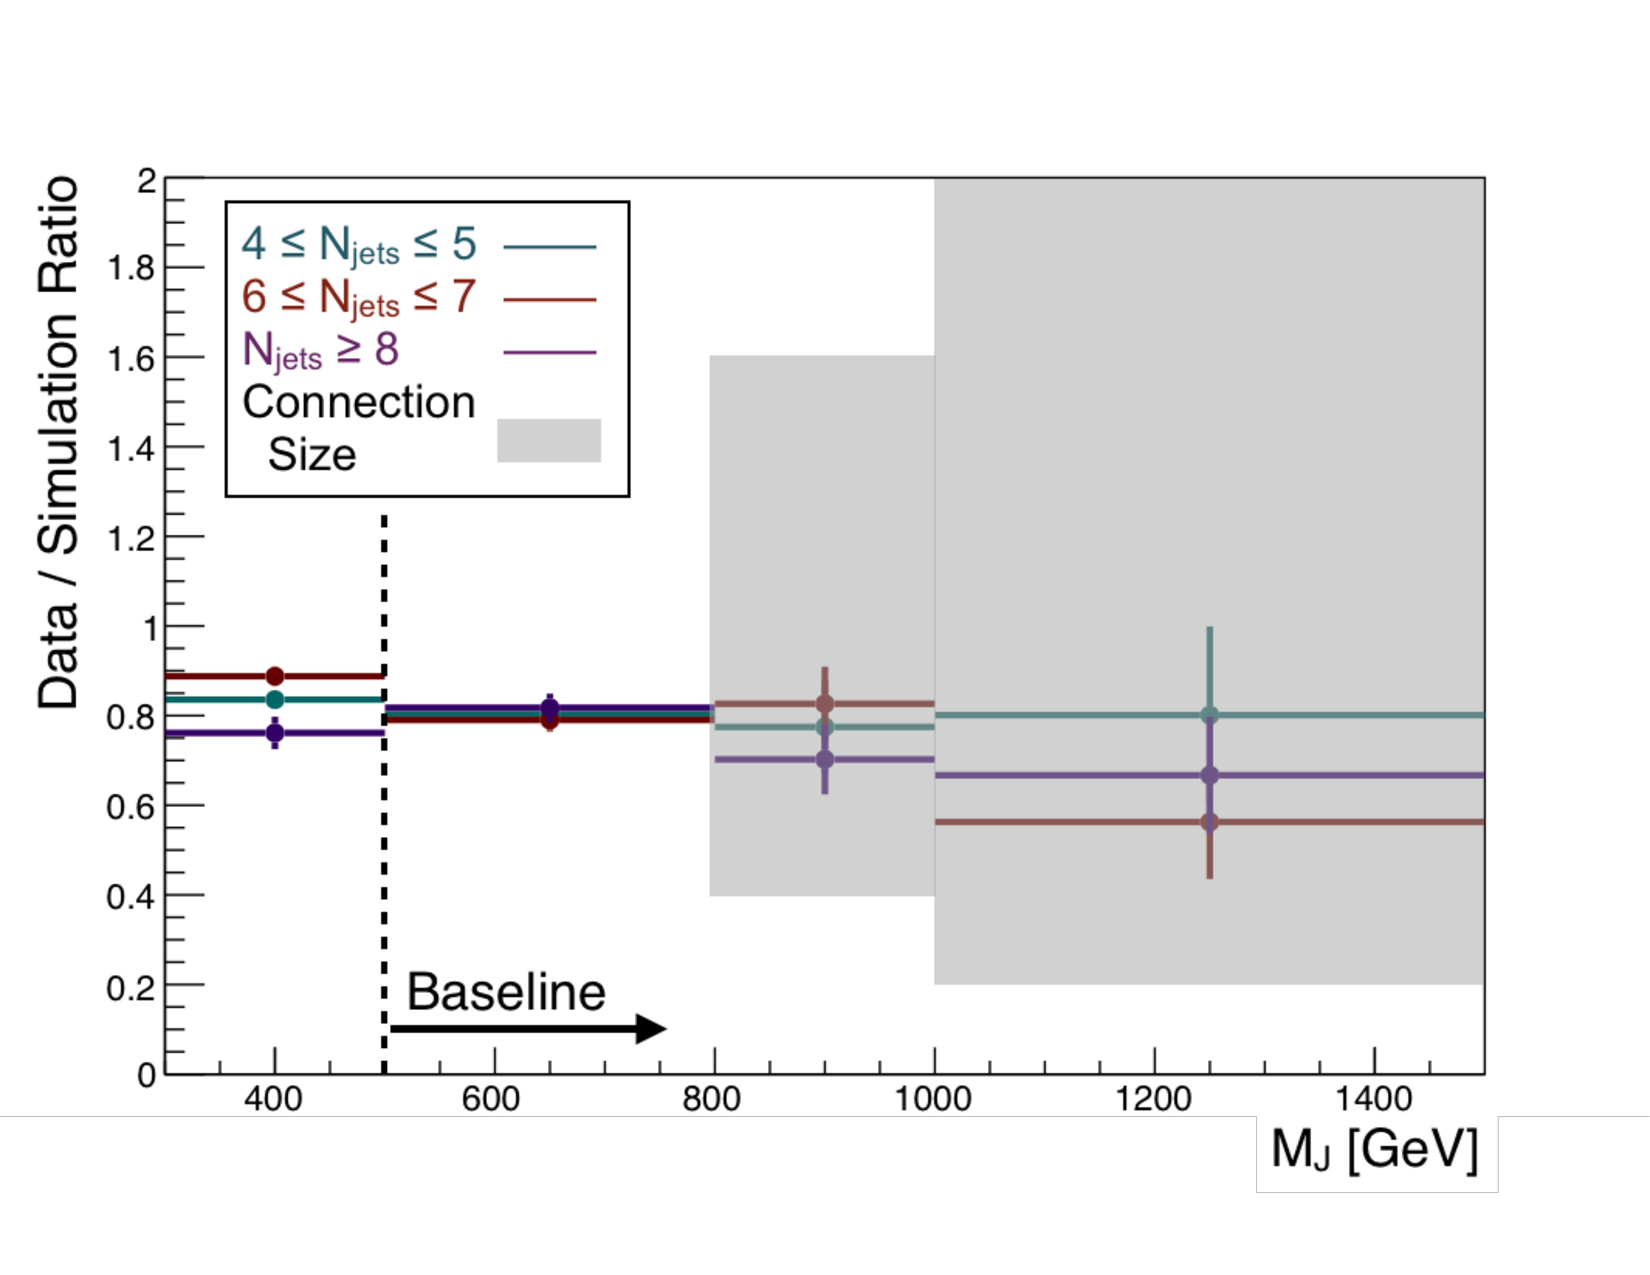
\includegraphics[angle=0,width=0.60\columnwidth]{fig/mj_connection.pdf}
\caption{Data-to-simulation ratios as a function of \MJ for different \Njets bins (data points) with a selection of $\Nleps = 1$, $\HT > 1200~\GeV$, and $\Nb = 1$ applied.
The shaded region corresponds to the size of the \MJ connection in each \MJ bin.}
\label{fig:mj_connection}
\end{figure}

\end{subsection}

\end{section}

\begin{section}{\Wjets Normalization}

The \Wjets background is determined in the fit with one global normalization parameter and two parameters to adjust the bin-to-bin normalization of adjacent \Njets bins, since the \Njets sahpe may not be well-modelled by simulation.
The amount the \Njets shape may vary is based on the data-to-simulation agreement in a kinematically similar \Zjets sample selected with $\Nleps = 2$ ($\mathrm{ee}$ or $\mu\mu$), $\HT > 1200~\GeV$, $\MJ > 500~\GeV$, $\Nb = 1$, and $80 < \mll < 100~\GeV$, where $\mll$ is the invariant mass of the two leptons.
The \Njets distribution and data/simulation yields ratio for this sample are shown in Figure~\ref{fig:njets_dy}.
The resulting variation sizes are 17\% between $4 \leq \Njets \leq 5$ and $6 \leq \Njets \leq 7$ and 62\% between $6 \le \Njets \le 7$ and $\Njets \ge8$.
After correcting the \Njets spectrum, the residual \MJ mismodeling is expected to be small, so no further correction is applied.

\begin{figure}[tbp!]
\centering
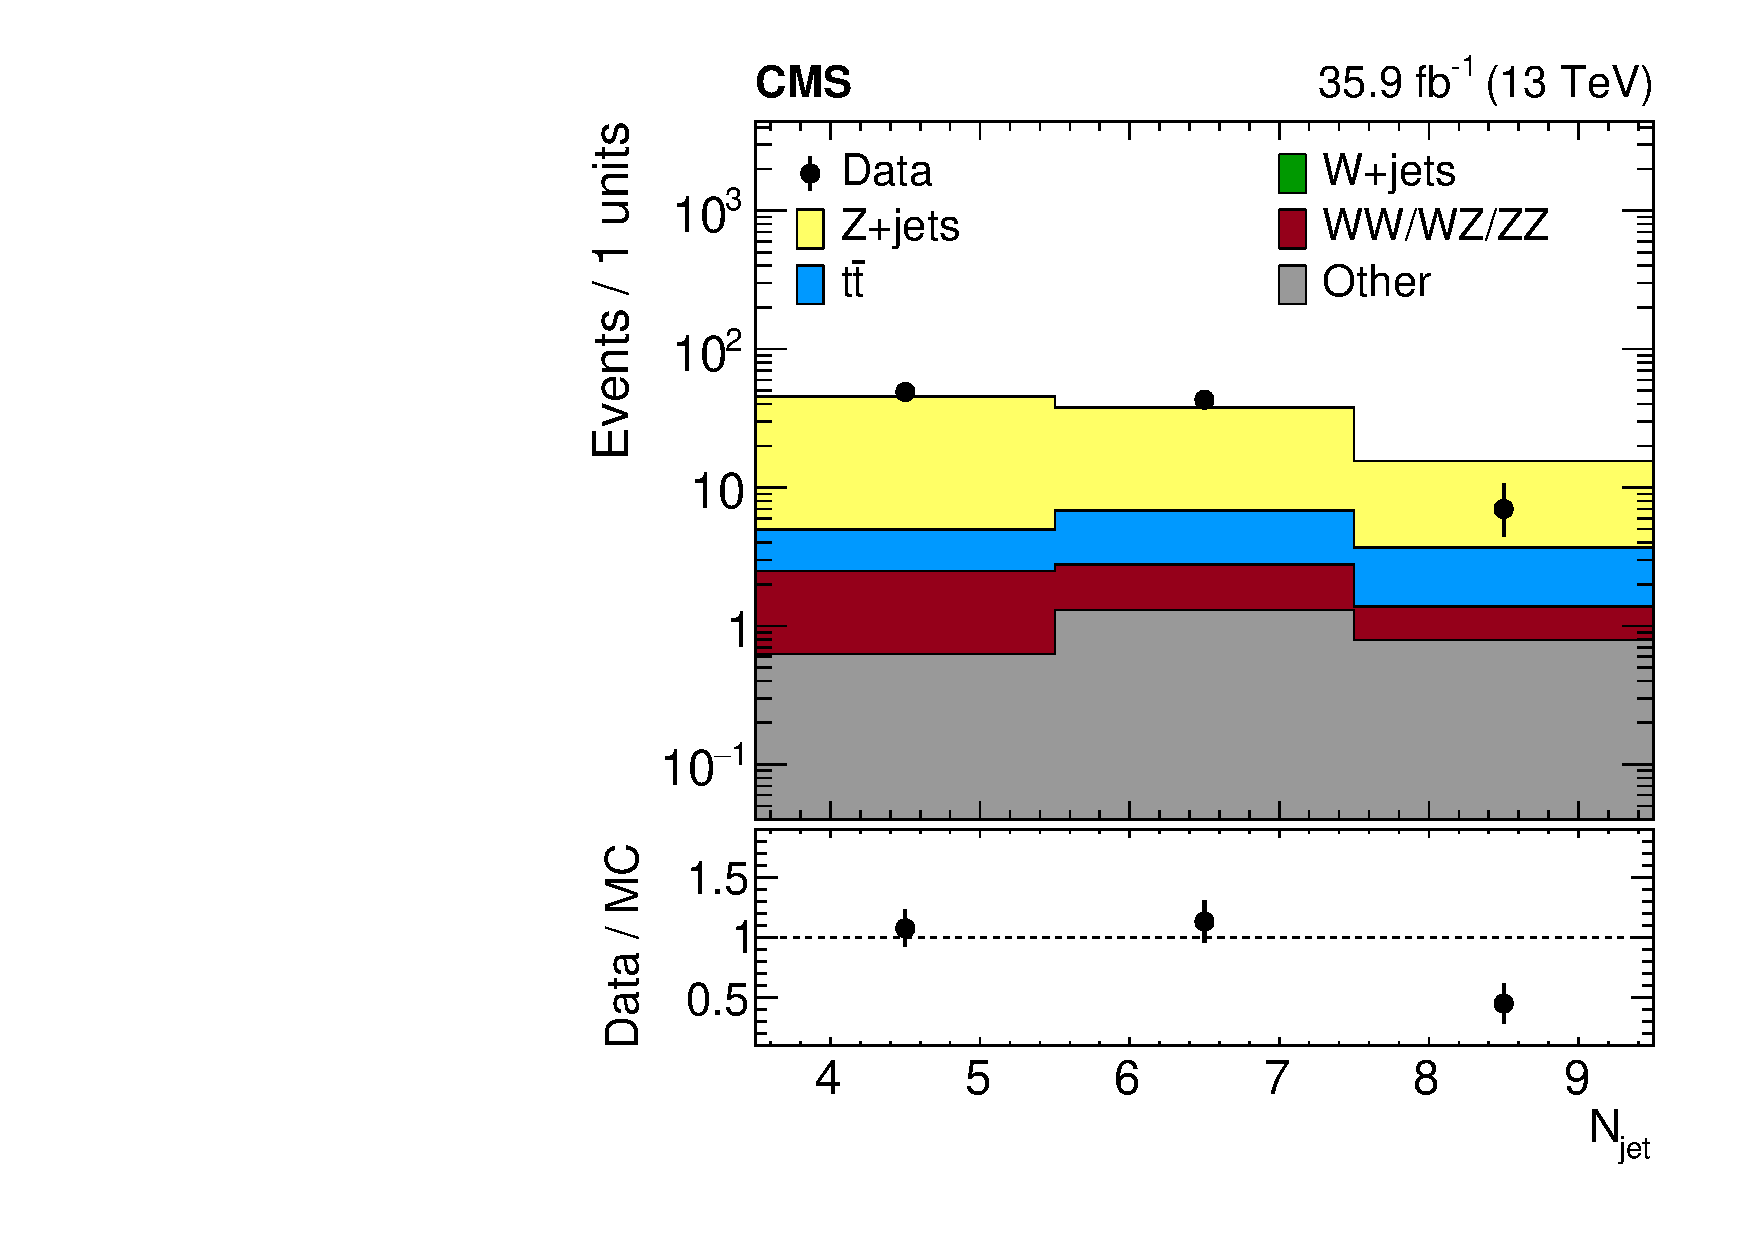
\includegraphics[angle=0,width=0.60\columnwidth]{fig/njets_dy.pdf}
\caption{Jet multiplicity distribution for data and simulation in a \Zjets control sample selected by requiring $\Nleps = 2$, $\HT > 1200~\GeV$, $\MJ > 500~\GeV$, $\Nb = 1$, and $80 < \mll < 100~\GeV$.
The total yield from simulation is normalized to the number of events in data.
The uncertainty in the ratio of data to simulation yields (lower panel) is statistical only.}
\label{fig:njets_dy}
\end{figure}

\end{section}

\begin{section}{Other Normalization}

The nominal normalization for Other is largely taken from simulation, as its contribution is less than 20\% in every bin with typical values $\lesssim 5\%$.
It is, however, allowed to vary according to statistical and systematic uncertainties.

\end{section}
